\PassOptionsToPackage{unicode=true}{hyperref} % options for packages loaded elsewhere
\PassOptionsToPackage{hyphens}{url}
%
\documentclass[11pt,ignorenonframetext,]{beamer}
\usepackage{pgfpages}
\setbeamertemplate{caption}[numbered]
\setbeamertemplate{caption label separator}{: }
\setbeamercolor{caption name}{fg=normal text.fg}
\beamertemplatenavigationsymbolsempty
\usepackage{lmodern}
\usepackage{amssymb,amsmath}
\usepackage{ifxetex,ifluatex}
\usepackage{fixltx2e} % provides \textsubscript
\ifnum 0\ifxetex 1\fi\ifluatex 1\fi=0 % if pdftex
  \usepackage[T1]{fontenc}
  \usepackage[utf8]{inputenc}
  \usepackage{textcomp} % provides euro and other symbols
\else % if luatex or xelatex
  \usepackage{unicode-math}
  \defaultfontfeatures{Ligatures=TeX,Scale=MatchLowercase}
\fi
\usetheme[]{Montpellier}
\usecolortheme{beaver}
% use upquote if available, for straight quotes in verbatim environments
\IfFileExists{upquote.sty}{\usepackage{upquote}}{}
% use microtype if available
\IfFileExists{microtype.sty}{%
\usepackage[]{microtype}
\UseMicrotypeSet[protrusion]{basicmath} % disable protrusion for tt fonts
}{}
\IfFileExists{parskip.sty}{%
\usepackage{parskip}
}{% else
\setlength{\parindent}{0pt}
\setlength{\parskip}{6pt plus 2pt minus 1pt}
}
\usepackage{hyperref}
\hypersetup{
            pdftitle={Performance comparison of the discrete choice models of consumer choice},
            pdfborder={0 0 0},
            breaklinks=true}
\urlstyle{same}  % don't use monospace font for urls
\newif\ifbibliography
% Prevent slide breaks in the middle of a paragraph:
\widowpenalties 1 10000
\raggedbottom
\setbeamertemplate{part page}{
\centering
\begin{beamercolorbox}[sep=16pt,center]{part title}
  \usebeamerfont{part title}\insertpart\par
\end{beamercolorbox}
}
\setbeamertemplate{section page}{
\centering
\begin{beamercolorbox}[sep=12pt,center]{part title}
  \usebeamerfont{section title}\insertsection\par
\end{beamercolorbox}
}
\setbeamertemplate{subsection page}{
\centering
\begin{beamercolorbox}[sep=8pt,center]{part title}
  \usebeamerfont{subsection title}\insertsubsection\par
\end{beamercolorbox}
}
\AtBeginPart{
  \frame{\partpage}
}
\AtBeginSection{
  \ifbibliography
  \else
    \frame{\sectionpage}
  \fi
}
\AtBeginSubsection{
  \frame{\subsectionpage}
}
\setlength{\emergencystretch}{3em}  % prevent overfull lines
\providecommand{\tightlist}{%
  \setlength{\itemsep}{0pt}\setlength{\parskip}{0pt}}
\setcounter{secnumdepth}{0}

% set default figure placement to htbp
\makeatletter
\def\fps@figure{htbp}
\makeatother

% Colors
% \usepackage{colortbl}

% Change section names style
\titlegraphic{
  \vspace{-20mm}
  \flushright
  \includegraphics[height = 8mm]{../images/lig_logo_1.png}
  \includegraphics[height = 8mm]{../images/gael_logo_3.jpg}
  \includegraphics[height = 8mm]{../images/uga_logo.png} 
}

%%%%%%%%%%%%%%%%%
% Load Packages %
%%%%%%%%%%%%%%%%%

% Spacings
\usepackage{setspace}

% Tables
\usepackage{longtable}
\usepackage{tabu}

% Floats
\usepackage{morefloats}
\usepackage{float}
\usepackage{placeins}

% Highlighting
\usepackage{soul}

% Horizontal page position
\usepackage{pdflscape}

% Append pdfs
\usepackage{pdfpages}

% Add latex chunks
\usepackage{docmute}

% Short toc
\usepackage{shorttoc}
%\setcounter{tocdepth}{1}
%\usepackage{minitoc} - incompatible with document class

% Referencing mutliple things with a single command - \cref
\usepackage{cleveref}

% Array
\usepackage{array}

% Multiple columns
\usepackage{multicol}

% Image insertion and colors
\usepackage{graphicx}

% Latex comments
\newenvironment{dummy}{}{}

% Fonts
% \usepackage{fontspec}
% \setmainfont{Museo}

% drawing
\usepackage{tikz}
\usetikzlibrary{matrix,chains,positioning,decorations.pathreplacing,arrows}

\usepackage{dcolumn}
% \usepackage{subfig}
\usepackage[export]{adjustbox}
% \usepackage[demo]{graphicx}  
\usepackage{subcaption}
\usetikzlibrary{shapes,arrows}
\usetikzlibrary{arrows.meta}
\usepackage[edges]{forest}

\usepackage{calc}


% Add footline
\makeatletter
\setbeamertemplate{footline}{%
  \leavevmode%
  \hbox{%
  \begin{beamercolorbox}[wd=.333333\paperwidth,ht=2.25ex,dp=1ex,center]{author in head/foot}%
    \usebeamerfont{author in head/foot}{Nikita Gusarov}
  \end{beamercolorbox}%
  \begin{beamercolorbox}[wd=.333333\paperwidth,ht=2.25ex,dp=1ex,center]{title in head/foot}%
    \usebeamerfont{institute in head/foot}\insertshortdate
  \end{beamercolorbox}%
  \begin{beamercolorbox}[wd=.333333\paperwidth,ht=2.25ex,dp=1ex,right]{date in head/foot}%
    \usebeamerfont{date in head/foot}\insertshortinstitute{}\hspace*{1em}
   %\insertframenumber{} / \inserttotalframenumber\hspace*{2ex} % old version
    \insertframenumber{} \hspace*{2ex} % new version without total frames
  \end{beamercolorbox}}%
  \vskip0pt%
}
\makeatother

\title{Performance comparison of the discrete choice models of consumer choice}
\providecommand{\subtitle}[1]{}
\subtitle{Exploration of the Econometrics and Machine Learning model performances
in the presence of heterogeneous preferences and random effects
utilities}
\author{Nikita Gusarov\\
\scriptsize M2 MIASHS C2ES (UGA)\\
~\\
\raggedright\scriptsize Under supervision of:\\
\raggedright\hspace{10mm}\scriptsize Iragaël Joly, HDR (GAEL, UGA,
Grenoble INP)\\
\raggedright\hspace{10mm}\scriptsize Beatrice Roussillon, MCF (GAEL,
UGA)}
\date{28/08/2020}

\begin{document}
\frame{\titlepage}

\hypertarget{introduction}{%
\section{Introduction}\label{introduction}}

\#\#~Presentation plan

\begin{itemize}
\tightlist
\item
  Background of the study
\item
  Methodology
\item
  Results presentation
\item
  Conclusion and future work
\end{itemize}

\begin{frame}{History (Hensher, Rose, and Greene 2015)}
\protect\hypertarget{history-hensher2015}{}

In economics and econometrics of the individual choice modelling the
\textcolor{red}{traditional scientific procedure} includes:

\begin{enumerate}
\tightlist
\item
  Economics question to resolve
\item
  Theoretical modelling of the underlying processus
\item
  Data collection (potentially through a controlled experiment)
\item
  Econometrics model estimation based on the theoretical counterpart
\end{enumerate}

\end{frame}

\begin{frame}{Scientific question of the study}
\protect\hypertarget{scientific-question-of-the-study}{}

\emph{``How can we \textcolor{red}{assess and compare the performances}
of different models applied to
\textcolor{red}{discrete consumer choice modelling} ?''}

This question becomes extremely complex when extended to the general
comparison of \emph{\textcolor{red}{Econometrics}} and
\emph{\textcolor{red}{Machine Learning (ML)}} models.

\end{frame}

\begin{frame}{Econometrics against ML (Breiman and others 2001)}
\protect\hypertarget{econometrics-against-ml-breiman2001stat}{}

\begin{figure}[hbtp]
\centering
\label{fig:parad}
\begin{subfigure}[c]{.4\linewidth}
    \centering
    \caption{Real world}
    \label{fig:parad1}
    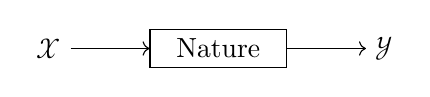
\begin{tikzpicture}[box/.style = {draw, text width=1.5cm, align=center}]
        \node[box] (b) {Nature};
        \node[left=of b] (a) {$\mathcal{X}$};
        \node[right=of b] (c) {$\mathcal{Y}$};
        \draw[->] (a) -- (b);
        \draw[->] (b) -- (c);
    \end{tikzpicture}
\end{subfigure}\vspace{12pt}

\begin{subfigure}[c]{.3\textwidth}
    \centering
    \caption{Econometrics}
    \label{fig:parad2}
    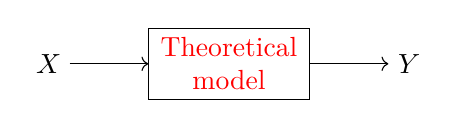
\begin{tikzpicture}[box/.style = {draw, text width=1.8cm, align=center}]
        \node[box] (b) {\textcolor{red}{Theoretical\\model}};
        \node[left=of b] (a) {$X$};
        \node[right=of b] (c) {$Y$};
        \draw[->] (a) -- (b);
        \draw[->] (b) -- (c);
    \end{tikzpicture}
\end{subfigure}
\hfill
\begin{subfigure}[c]{.3\linewidth}
    \centering
    \caption{Machine learning}
    \label{fig:parad3}
    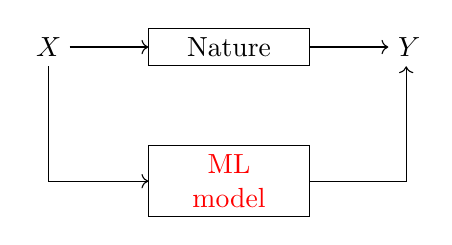
\begin{tikzpicture}[box/.style = {draw, text width=1.8cm, align=center}]
        \node[box] (b) {Nature};
        \node[box, below=of b] (d) {\textcolor{red}{ML\\model}};
        \node[left=of b] (a) {$X$};
        \node[right=of b] (c) {$Y$};
        \draw[->] (a) -- (b);
        \draw[->] (b) -- (c);
        \draw[->] (a) |- (d);
        \draw[->] (d) -| (c);
    \end{tikzpicture}
\end{subfigure}
\hspace{2cm}
\end{figure}

\end{frame}

\begin{frame}{Objectives}
\protect\hypertarget{objectives}{}

Theoretical:

\begin{itemize}
\tightlist
\item
  \emph{Offer a comprehensive \textcolor{red}{methodology} for consumer
  choice models comparison}
\item
  \emph{Devise a \textcolor{red}{framework} which will allow to test
  hypotheses affecting modelling and model performances}
\item
  \emph{\textcolor{red}{Test the proposed framework} on a real world
  problematic}
\end{itemize}

Applied:

\begin{itemize}
\tightlist
\item
  \emph{Study the \textcolor{red}{effects of heterogeneous preferences}
  in population on the estimation results}
\end{itemize}

\end{frame}

\begin{frame}{Scientific procedure}
\protect\hypertarget{scientific-procedure}{}

In this study we:

\begin{enumerate}
\tightlist
\item
  Propose a \textcolor{red}{theory-testing framework}
\item
  Explore the different \textcolor{red}{models' performances} in the
  presence of \textcolor{red}{heterogeneous preferences} for attributes
  in population using the designed framework
\end{enumerate}

Which involves:

\begin{itemize}
\tightlist
\item
  Construction of \textcolor{red}{two artificial datasets} controlling
  for the presence of \textcolor{red}{heterogeneous} and
  \textcolor{red}{homogeneous} preferences in population
\item
  Estimation of a selection of \textcolor{red}{three models}, issued
  from \emph{econometrics} and \emph{ML}, over the generated datasets
\item
  \textcolor{red}{Evaluation of the performances} of the models over
  multiple criterias
\end{itemize}

\end{frame}

\hypertarget{methodology}{%
\section{Methodology}\label{methodology}}

\begin{frame}{Proposed framework}
\protect\hypertarget{proposed-framework}{}

\begin{figure}
    \centering
    \label{fig:burel}
    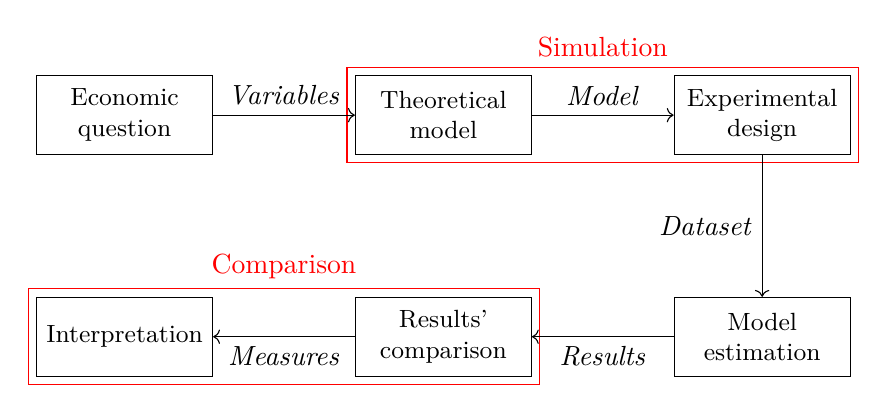
\begin{tikzpicture}[
        box/.style = {
            draw, 
            text width=2cm, 
            align=center, 
            minimum width={width("Interpretation")+2pt},
            minimum height={1cm},
            font=\small
        },node distance=1.8cm]

        \node[box] (b) {Theoretical\\model};
        \node[box, left=of b] (a) {Economic\\question};
        \node[box, right=of b] (c) {Experimental\\design};
        \node[box, below=of c] (d) {Model\\estimation};
        \node[box, below=of b] (e) {Results'\\comparison};
        \node[box, below=of a] (f) {Interpretation};

        \node[rectangle, draw=red, fit=(b) (c), inner sep=1mm, label=above:{\textcolor{red}{Simulation}}] (bc) {};
        \node[rectangle, draw=red, fit=(e) (f), inner sep=1mm, label=above:{\textcolor{red}{Comparison}}] (ef) {};
        
        \draw[->] (a) -- (b) node[midway, above] {\textit{Variables}};
        \draw[->] (b) -- (c) node[midway, above] {\textit{Model}};
        \draw[->] (c) -- (d) node[midway, left] {\textit{Dataset}};
        \draw[->] (d) -- (e) node[midway, below] {\textit{Results}};
        \draw[->] (e) -- (f) node[midway, below] {\textit{Measures}};
    \end{tikzpicture}
\end{figure}

\end{frame}

\begin{frame}{Consumer choice modelling (McFadden 1974)}
\protect\hypertarget{consumer-choice-modelling-mcfadden1974utd}{}

Alternatives' set, from which only one alternative may be chosen

\begin{equation}
\{\omega_1, \dots, \omega_r \} \in \Omega
\end{equation}

Utility definition incorporating fixed and random terms, with
\(i \in \{1, ..., N\}\) and \(j \in \Omega\)

\begin{equation}
U_{ij} = V_{ij} + \eta_{ij} \text{  where  } V_{ij} = f(X_i, Z_j)
\end{equation}

Random utility specification

\begin{equation}
\eta_{ij} \sim Gumble(0, 1)
\end{equation}

\end{frame}

\begin{frame}{Models implemented}
\protect\hypertarget{models-implemented}{}

\small
\begin{table}[!htbp] \centering 
 \label{tab:comb1} 
\begin{tabular}{@{\extracolsep{5pt}}lp{70mm}} 
\\[-1.8ex]\hline 
\hline \\[-1.8ex] 
Model & \multicolumn{1}{c}{Characteristics} \\ 
\hline \\[-1.8ex] 
MMNL & 
    \textcolor{red}{Advanced} model used to estimate complex relationships \newline 
    \textit{Ex: random effects modelling} \\
MNL & 
    One of the most \textcolor{red}{popular} models in economics for treatment of multiple choice situations \newline 
    \textit{This leads to potential biases in many contemporary studies} \\
CNN & 
    Model with \textcolor{red}{flexible} architecture specifically adjusted for the studied case \newline 
    \textit{The computational efficiency offered by Big data techniques makes it particularly interesting} \\
\hline \\[-1.8ex] 
\end{tabular} 
\end{table} 
\normalsize

\end{frame}

\begin{frame}{Traditional NN design}
\protect\hypertarget{traditional-nn-design}{}

\begin{figure}[htp]
\centering
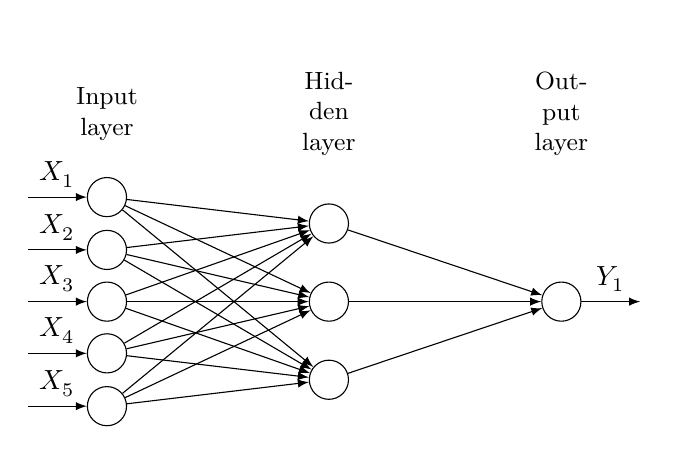
\begin{tikzpicture}[
    plain/.style={
        draw = none,
        fill = none,
        font = \small
    },
    net/.style={
        matrix of nodes,
        nodes={
            draw,
            circle,
            inner sep = 5pt,
            font = \tiny
        },
        nodes in empty cells,
        column sep = 1cm,
        row sep = -5pt,
        ampersand replacement=\&
    },
    >=latex
    ]
    
\matrix[net] (mat)
{
    |[plain]| \parbox{1cm}{\centering Input\\layer} \& |[plain]| \parbox{1cm}{\centering Hidden\\layer} \& |[plain]| \parbox{1cm}{\centering Output\\layer} \\
    \& |[plain]| \\
    |[plain]| \& \\
    \& |[plain]| \\
    |[plain]| \& |[plain]| \\
    \& \& \\
    |[plain]| \& |[plain]| \\
    \& |[plain]| \\
    |[plain]| \& \\
    \& |[plain]| \\
};

\foreach \ai [count=\mi ]in {2,4,...,10}
    \draw[<-] (mat-\ai-1) -- node[above] {$X_{\mi}$} +(-1cm,0);
\foreach \ai in {2,4,...,10}
{\foreach \aii in {3,6,9}
    \draw[->] (mat-\ai-1) -- (mat-\aii-2);
}
\foreach \ai in {3,6,9}
    \draw[->] (mat-\ai-2) -- (mat-6-3);
\draw[->] (mat-6-3) -- node[above] {$Y_1$} +(1cm,0);
\end{tikzpicture}
\end{figure}

\end{frame}

\begin{frame}{Chosen CNN design}
\protect\hypertarget{chosen-cnn-design}{}

\small
\begin{figure}[!htbp] \centering 
 \label{fig:cnn} 
\small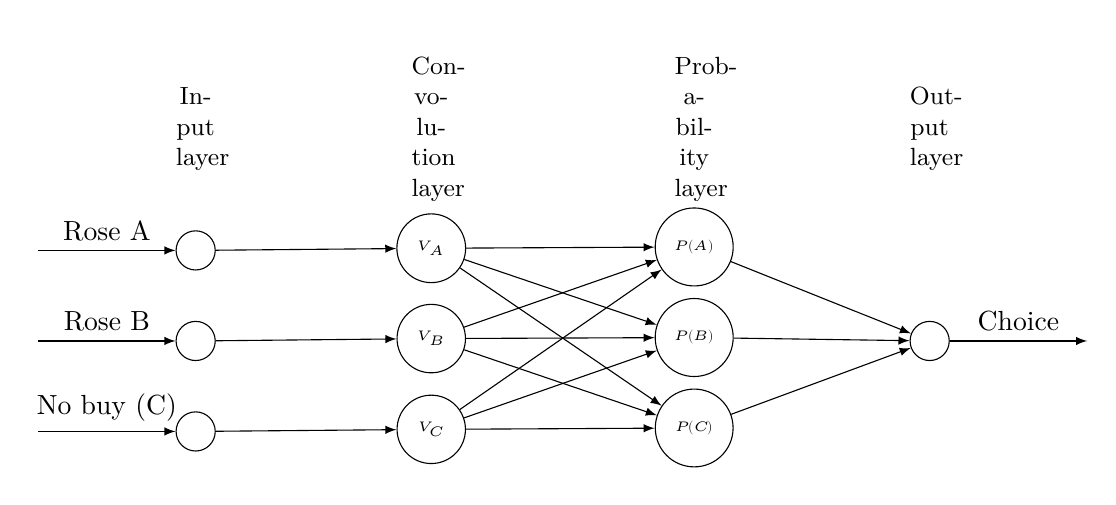
\begin{tikzpicture}[
    plain/.style={
        draw = none,
        fill = none,
        font = \small
    },
    net/.style={
        matrix of nodes,
        nodes={
            draw,
            circle,
            inner sep = 5pt,
            font = \tiny
        },
        nodes in empty cells,
        column sep = 1cm,
        row sep = -5pt,
        ampersand replacement=\&
    },
    >=latex 
]

\matrix[net] (mat)
{
    |[plain]| \parbox{0.5cm}{\centering Input\\layer} \& 
        |[plain]| \parbox{0.5cm}{\centering Convolution\\layer} \& 
        |[plain]| \parbox{0.5cm}{\centering Probability\\layer} \& 
        |[plain]| \parbox{0.5cm}{\centering Output\\layer} \\
    \& $V_A$ \& $P(A)$ \& |[plain]| \\
        |[plain]| \& |[plain]| \& |[plain]| \\
    \& $V_B$ \& $P(B)$ \& \\
        |[plain]| \& |[plain]| \& |[plain]| \\
    \& $V_C$ \& $P(C)$ \& |[plain]| \\
};


\draw[<-] (mat-2-1) -- node[above] {Rose A} +(-2cm,0);
\draw[<-] (mat-4-1) -- node[above] {Rose B} +(-2cm,0);
\draw[<-] (mat-6-1) -- node[above] {No buy (C)} +(-2cm,0);
\foreach \ai in {2,4,6}
    \draw[->] (mat-\ai-1) -- (mat-\ai-2);
\foreach \ai in {2,4,6}
    {\foreach \aii in {2,4,6}
        \draw[->] (mat-\ai-2) -- (mat-\aii-3);
    }
\foreach \ai in {2,4,6}
    \draw[->] (mat-\ai-3) -- (mat-4-4);
\draw[->] (mat-4-4) -- node[above] {Choice} +(2cm,0);

\end{tikzpicture}
\end{figure}
\normalsize

\end{frame}

\begin{frame}{Performance comparison}
\protect\hypertarget{performance-comparison}{}

\begin{itemize}
\tightlist
\item
  Precision in derivation of the economics values

  \begin{itemize}
  \tightlist
  \item
    Underlying \textcolor{red}{parameters} of the utility function
  \item
    Case specific economic targets (WTP, Premiums, \ldots{})
  \end{itemize}
\item
  \textcolor{red}{Overall fit} performance metrics

  \begin{itemize}
  \tightlist
  \item
    Absolute measures (Accuracy, \ldots{})
  \item
    Probabilistic measures (KLD, \ldots{})
  \end{itemize}
\item
  \textcolor{red}{Alternative-specific} performance metrics

  \begin{itemize}
  \tightlist
  \item
    Simple measures (TPR, TNR, \ldots{})
  \item
    Derived measures (F-measure, Geometric means, \ldots{})
  \end{itemize}
\item
  Technical efficiency and \textcolor{red}{ressources consumption}

  \begin{itemize}
  \tightlist
  \item
    Estimation time
  \end{itemize}
\end{itemize}

\end{frame}

\begin{frame}{The starting point}
\protect\hypertarget{the-starting-point}{}

\emph{We would like to \textcolor{red}{demonstrate} the advantages of
our framework studying how \textcolor{red}{heterogeneous preferences} in
population affect the results}

Using an existing application (Michaud, Llerena, and Joly 2012), which
incorporates all the elements of the framework:

\begin{itemize}
\tightlist
\item
  Economics question -
  \textcolor{red}{individual preferences for environmental attributes in presence of heterogenous preferences}
\item
  Behavioural assumptions -
  \textcolor{red}{random utility maximisation theory}
\item
  Experimental design -
  \textcolor{red}{complex factorial design with random price allocation}
\item
  Advanced model implemented to model individual choices -
  \textcolor{red}{mixed logit}
\item
  Economics target values -
  \textcolor{red}{willingness to pay for environmental attributes}
\end{itemize}

\end{frame}

\begin{frame}{Utility function specification (Michaud, Llerena, and Joly
2012)}
\protect\hypertarget{utility-function-specification-llerena2013rose}{}

Deterministic utility of the ``Buy'' option is

\begin{align}
V_{ij} = & \nonumber \\
    & \alpha_{i,Buy} + \nonumber \\
    & \textcolor{red}{\beta_{Buy, Sex}} Sex_i + \textcolor{red}{\beta_{Buy, Age}} Age_i + \nonumber \\
    & \textcolor{red}{\beta_{Buy, Income}} Income_i + \textcolor{red}{\beta_{Buy, Habit}} Habit_i + \\
    & \textcolor{blue}{\gamma_{Price}} Price_{ij} + \textcolor{blue}{\gamma_{i, Label}} Label_{ij} + \nonumber \\ 
    & \textcolor{blue}{\gamma_{i, Carbon}} Carbon_{ij} + \textcolor{blue}{\gamma_{i, Label \times Carbon}} Label_{ij} \times Carbon_{ij} \nonumber 
\end{align}

\scriptsize

Where \(i \in \{1, \dots, N\}\),
\(j \in \{\text{"Buy A"}, \text{"Buy B"}, \text{"No buy"}\}\) and
\(Buy = I(j \in \{\text{"Buy A"}, \text{"Buy B"}\})\). \normalsize 

\end{frame}

\begin{frame}{Target values from Michaud, Llerena, and Joly (2012)}
\protect\hypertarget{target-values-from-llerena2013rose}{}

\scriptsize
\begin{table}[!htbp]\centering
    \label{tab:params}
\hspace{-2cm}\begin{subfigure}[l]{.3\linewidth}
    \centering
    \label{tab:params1}
\begin{tabular}[b]{@{\extracolsep{5pt}}lc} 
\\[-1.8ex]\hline 
\hline \\[-1.8ex] 
& \multicolumn{1}{c}{\textit{Effects}} \\ 
\cline{2-2} 
\\[-1.8ex] & \multicolumn{1}{c}{\textit{Means}} \\
\hline \\[-1.8ex] 
\textbf{Individual characteristics (\textcolor{red}{$\beta$})} & \\
    ~~~Sex $\textcolor{red}{\beta_{Buy, Sex}}$ & 1.420 \\ 
    ~~~Age $\textcolor{red}{\beta_{Buy, Age}}$ & 0.009 \\ 
    ~~~Salary $\textcolor{red}{\beta_{Buy, Income}}$ & 0.057 \\ 
    ~~~Habit $\textcolor{red}{\beta_{Buy, Habit}}$ & 1.027 \\ 
\textbf{Alternatives' attributes (\textcolor{blue}{$\gamma$, $\alpha$)}} & \\
    ~~~Price $\textcolor{blue}{\gamma_{Price}}$ & $-$1.631 \\ 
    ~~~Label $\textcolor{blue}{\gamma_{i, Label}}$ & 2.824 \\ 
    ~~~Carbon $\textcolor{blue}{\gamma_{i, Carbon}}$ & 6.665 \\ 
    ~~~LC $\textcolor{blue}{\gamma_{i, Label \times Carbon}}$ & $-$2.785 \\
    ~~~Buy $\alpha_{i,Buy}$ & 2.285 \\ 
    ~~~ & \\
\hline \\[-1.8ex] 
\end{tabular} 
\end{subfigure}
\hspace{3cm}\begin{subfigure}[r]{.3\linewidth}
    \centering
    \label{tab:params2}
\begin{tabular}{@{\extracolsep{5pt}}lcc} 
\\[-1.8ex]\hline 
\hline \\[-1.8ex] 
 & \multicolumn{2}{c}{\textit{Effects}} \\ 
\cline{2-3} 
\\[-1.8ex] & Fixed & Random \\ 
\hline \\[-1.8ex] 
\textbf{Variance} & & \\
    ~~~Buy & 0 & 3.202 \\  
    ~~~Label & 0 & 2.654 \\  
    ~~~Carbon & 0 & 3.535 \\  
    ~~~LC & 0 & 2.711 \\ 
\textbf{Covariance} & & \\ 
    ~~~Buy:Label & 0 & -0.54 \\  
    ~~~Buy:Carbon & 0 & -4.39 \\  
    ~~~Buy:LC & 0 & 6.17 \\  
    ~~~Label:Carbon & 0 & 8.77 \\  
    ~~~Label:LC & 0 & -2.33 \\  
    ~~~Carbon:LC & 0 & -4.82 \\ 
\hline \\[-1.8ex] 
\end{tabular} 
\end{subfigure}
\end{table}
\normalsize

\end{frame}

\hypertarget{results}{%
\section{Results}\label{results}}

\begin{frame}{Simulated datasets: Individuals}
\protect\hypertarget{simulated-datasets-individuals}{}

\scriptsize

\begin{table}[!htbp] \centering 
\begin{tabular}{@{\extracolsep{5pt}}lcccr}
\\[-1.8ex]\hline 
\hline \\[-1.8ex] 
 & Fixed Effects  & Random Effects  & Target  & p value\\
 & (N=1000) & (N=1000) & (N=102) &  \\
\hline \\[-1.8ex] 
\textbf{Sex} &  &  &  & 0.851\\
~~~Mean (SD) & 0.506 (0.500) & 0.515 (0.500) & 0.490 (0.502) & \\
~~~Range & 0.000 - 1.000 & 0.000 - 1.000 & 0.000 - 1.000 & \\
\textbf{Habit} &  &  &  & 0.182\\
~~~N-Miss & 0 & 0 & 1 & \\
~~~Mean (SD) & 0.683 (0.466) & 0.657 (0.475) & 0.604 (0.492) & \\
~~~Range & 0.000 - 1.000 & 0.000 - 1.000 & 0.000 - 1.000 & \\
\textbf{Salary} &  &  &  & < 0.001\\
~~~Mean (SD) & 2.750 (1.476) & 2.671 (1.438) & 2.147 (1.222) & \\
~~~Range & 1.000 - 6.000 & 1.000 - 6.000 & 1.000 - 6.000 & \\
\textbf{Age} &  &  &  & 0.255\\
~~~Mean (SD) & 41.862 (13.685) & 42.161 (13.820) & 39.755 (18.895) & \\
~~~Range & 18.000 - 84.000 & 18.000 - 84.000 & 18.000 - 85.000 & \\
\hline
\end{tabular}
\end{table}
\normalsize

\end{frame}

\begin{frame}{Simulated datasets: Alternatives}
\protect\hypertarget{simulated-datasets-alternatives}{}

\scriptsize

\begin{table}[!htbp] \centering 
  \caption{Alternatives' descriptive statistics by dataset} 
\begin{tabular}{@{\extracolsep{5pt}}lcccr}
\\[-1.8ex]\hline 
\hline \\[-1.8ex] 
 & Fixed Effects  & Random Effects  & Target  & p value\\
 & (N=320000) & (N=320000) & (N=2372) &  \\
\hline \\[-1.8ex] 
\textbf{Price} &  &  &  & 0.002\\
~~~Mean (SD) & 2.936 (0.958) & 2.936 (0.958) & 3.005 (0.887) & \\
~~~Range & 1.500 - 4.500 & 1.500 - 4.500 & 1.500 - 4.500 & \\
\textbf{Carbon} &  &  &  & 0.999\\
~~~Mean (SD) & 0.500 (0.500) & 0.500 (0.500) & 0.500 (0.500) & \\
~~~Range & 0.000 - 1.000 & 0.000 - 1.000 & 0.000 - 1.000 & \\
\textbf{Label} &  &  &  & 0.999\\
~~~Mean (SD) & 0.500 (0.500) & 0.500 (0.500) & 0.500 (0.500) & \\
~~~Range & 0.000 - 1.000 & 0.000 - 1.000 & 0.000 - 1.000 & \\
\hline
\end{tabular}
\end{table}
\normalsize

\end{frame}

\begin{frame}{Estimates of mean effects}
\protect\hypertarget{estimates-of-mean-effects}{}

\tiny
\begin{table}[!htbp] \centering 
  \tiny
\begin{tabular}{@{\extracolsep{0pt}}l ccccccc } 
\\[-1.8ex]\hline 
\hline \\[-1.8ex] 
 & \multicolumn{3}{c}{\textcolor{red}{\textit{Fixed effects}}} & \multicolumn{3}{c}{\textit{Random effects}} & \multicolumn{1}{c}{\textcolor{red}{\textit{Target}}} \\ 
\cline{2-4}\cline{5-7} 
\\[-1.8ex] & \multicolumn{1}{c}{\textcolor{red}{MNL}} & \multicolumn{1}{c}{\textcolor{red}{MMNL}} & \multicolumn{1}{c}{CNN} & \multicolumn{1}{c}{MNL} & \multicolumn{1}{c}{MMNL} & \multicolumn{1}{c}{CNN} & \\ 
\hline \\[-1.8ex] 
\textbf{Characteristics} & & & & & & & \\ 
    ~~~Sex & $\mathbf{1.401}^{***}$ & $1.400^{***}$ & 1.369 & $0.712^{***}$ & $1.297^{***}$ & $0.719$ & $\mathbf{1.420}$ \\ 
    & (0.031) & (0.031) & & (0.016) & (0.024) & & \\ 
    ~~~Age & $\mathbf{0.009}^{***}$ & $\mathbf{0.009}^{***}$ & 0.010 & $0.007^{***}$ & $0.010^{***}$ & $0.005$ & $\mathbf{0.009}$ \\ 
    & (0.001) & (0.001) & & (0.001) & (0.001) & & \\ 
    ~~~Salary & $0.048^{***}$ & $0.048^{***}$ & $\mathbf{0.060}$ & $0.066^{***}$ & $0.120^{***}$ & $0.062$ & $\mathbf{0.057}$ \\ 
    & (0.010) & (0.010) & & (0.005) & (0.008) & & \\ 
    ~~~Habit & $1.070^{***}$ & $1.071^{***}$ & $\mathbf{1.056}$ & $0.361^{***}$ & $0.641^{***}$ & $0.343$ & $\mathbf{1.027}$ \\ 
    & (0.030) & (0.030) & & (0.016) & (0.024) & & \\ 
\textbf{Attributes} & & & & & & & \\ 
    ~~~Price & -$1.626^{***}$ & -$\mathbf{1.628}^{***}$ & -1.618 & -$0.886^{***}$ & -$1.586^{***}$ & -$0.886$ & -$\mathbf{1.631}$ \\ 
    & (0.010) & (0.010) & & (0.006) & (0.010) & & \\ 
    ~~~Buy & $\mathbf{2.311}^{***}$ & $2.313^{***}$ & 2.228 & $0.662^{***}$ & $2.180^{***}$ & $0.665$ & $\mathbf{2.285}$ \\ 
    & (0.065) & (0.066) & & (0.036) & (0.054) & & \\ 
    ~~~Label & $2.815^{***}$ & $\mathbf{2.817}^{***}$ & 2.810 & $1.279^{***}$ & $1.922^{***}$ & $1.277$ & $\mathbf{2.824}$ \\ 
    & (0.022) & (0.022) & & (0.015) & (0.023) & & \\ 
    ~~~Carbon & $6.654^{***}$ & $\mathbf{6.662}^{***}$ & 6.634 & $3.259^{***}$ & $5.430^{***}$ & $3.250$ & $\mathbf{6.665}$ \\ 
    & (0.032) & (0.033) & & (0.016) & (0.030) & & \\ 
    ~~~LC & -$2.781^{***}$ & -$\mathbf{2.782}^{***}$ & -2.765 & -$1.546^{***}$ & -$2.663^{***}$ & -$1.558$ & -$\mathbf{2.785}$ \\ 
    & (0.028) & (0.028) & & (0.019) & (0.030) & & \\ 
\hline 
\hline \\[-1.8ex] 
\textit{Note:}  & \multicolumn{7}{r}{$^{*}$p$<$0.1; $^{**}$p$<$0.05; $^{***}$p$<$0.01} \\ 
\end{tabular} 
\end{table} 
\normalsize

\end{frame}

\begin{frame}{Estimates of mean effects}
\protect\hypertarget{estimates-of-mean-effects-1}{}

\tiny
\begin{table}[!htbp] \centering 
  \tiny
\begin{tabular}{@{\extracolsep{0pt}}l ccccccc} 
\\[-1.8ex]\hline 
\hline \\[-1.8ex] 
 & \multicolumn{3}{c}{\textit{Fixed effects}} & \multicolumn{3}{c}{\textcolor{red}{\textit{Random effects}}} & \multicolumn{1}{c}{\textcolor{red}{\textit{Target}}} \\ 
\cline{2-4}\cline{5-7} 
\\[-1.8ex] & \multicolumn{1}{c}{MNL} & \multicolumn{1}{c}{MMNL} & \multicolumn{1}{c}{CNN} & \multicolumn{1}{c}{\textcolor{red}{MNL}} & \multicolumn{1}{c}{MMNL} & \multicolumn{1}{c}{\textcolor{red}{CNN}} & \\ 
\hline \\[-1.8ex] 
\textbf{Characteristics} & & & & & & & \\ 
    ~~~Sex & $1.401^{***}$ & $1.400^{***}$ & 1.369 & $0.712^{***}$ & $\mathbf{1.297^{***}}$ & $0.719$ & $\mathbf{1.420}$ \\ 
    & (0.031) & (0.031) & & (0.016) & (0.024) & & \\ 
    ~~~Age & $0.009^{***}$ & $0.009^{***}$ & 0.010 & $0.007^{***}$ & $\mathbf{0.010^{***}}$ & $0.005$ & $\mathbf{0.009}$ \\ 
    & (0.001) & (0.001) & & (0.001) & (0.001) & & \\ 
    ~~~Salary & $0.048^{***}$ & $0.048^{***}$ & 0.060 & $0.066^{***}$ & $0.120^{***}$ & $\mathbf{0.062}$ & $\mathbf{0.057}$ \\ 
    & (0.010) & (0.010) & & (0.005) & (0.008) & & \\ 
    ~~~Habit & $1.070^{***}$ & $1.071^{***}$ & 1.056 & $0.361^{***}$ & $\mathbf{0.641^{***}}$ & $0.343$ & $\mathbf{1.027}$ \\ 
    & (0.030) & (0.030) & & (0.016) & (0.024) & & \\ 
\textbf{Attributes} & & & & & & & \\ 
    ~~~Price & -$1.626^{***}$ & -$1.628^{***}$ & -1.618 & -$0.886^{***}$ & -$\mathbf{1.586^{***}}$ & -$0.886$ & -$\mathbf{1.631}$ \\ 
    & (0.010) & (0.010) & & (0.006) & (0.010) & & \\ 
    ~~~Buy & $2.311^{***}$ & $2.313^{***}$ & 2.228 & $0.662^{***}$ & $\mathbf{2.180^{***}}$ & $0.665$ & $\mathbf{2.285}$ \\ 
    & (0.065) & (0.066) & & (0.036) & (0.054) & & \\ 
    ~~~Label & $2.815^{***}$ & $2.817^{***}$ & 2.810 & $1.279^{***}$ & $\mathbf{1.922^{***}}$ & $1.277$ & $\mathbf{2.824}$ \\ 
    & (0.022) & (0.022) & & (0.015) & (0.023) & & \\ 
    ~~~Carbon & $6.654^{***}$ & $6.662^{***}$ & 6.634 & $3.259^{***}$ & $\mathbf{5.430^{***}}$ & $3.250$ & $\mathbf{6.665}$ \\ 
    & (0.032) & (0.033) & & (0.016) & (0.030) & & \\ 
    ~~~LC & -$2.781^{***}$ & -$2.782^{***}$ & -2.765 & -$1.546^{***}$ & -$\mathbf{2.663^{***}}$ & -$1.558$ & -$\mathbf{2.785}$ \\ 
    & (0.028) & (0.028) & & (0.019) & (0.030) & & \\ 
\hline 
\hline \\[-1.8ex] 
\textit{Note:}  & \multicolumn{7}{r}{$^{*}$p$<$0.1; $^{**}$p$<$0.05; $^{***}$p$<$0.01} \\ 
\end{tabular} 
\end{table} 
\normalsize

\end{frame}

\begin{frame}{Case specific metrics: WTP and Premiums}
\protect\hypertarget{case-specific-metrics-wtp-and-premiums}{}

\tiny
\begin{table}[!htbp] \centering  
    \label{tab:wtp}  
\begin{tabular}{@{\extracolsep{5pt}} lccc >{\boldmath\bfseries}cccc >{\boldmath\bfseries}c}  
\\[-1.8ex]\hline  
\hline \\[-1.8ex]  
& \multicolumn{4}{c}{\textit{Fixed effects}} & \multicolumn{4}{c}{\textit{Random effects}} \\
\cline{2-5}\cline{6-9} 
\\[-1.8ex] & \textcolor{red}{MNL} & MMNL & CNN & \textcolor{red}{Target} & \textcolor{red}{MNL} & MMNL & CNN & \textcolor{red}{Target} \\  
\hline \\[-1.8ex]  
WTP & $1.421$ & \textbf{1.416} & $1.377$ & $1.401$ & $0.747$ & \textbf{1.360} & $0.751$ & $1.401$ \\  
    & & (0.058) & & & & (1.887) & & (1.973) \\
Label & \textbf{1.731} & 1.732 & $1.737$ & $1.731$ & \textbf{1.445} & 1.243 & $1.442$ & $1.731$ \\  
    & & (0.019) & & & & (1.667) & & (1.611) \\
Carbon & \textbf{4.091} & 4.097 & $4.101$ & $4.086$ & \textbf{3.679} & 3.467 & $3.669$ & $4.086$ \\  
    & & (0.103) & & & & (2.323) & & (2.134) \\
LC & \textbf{4.112} & 4.116 & $4.129$ & $4.110$ & \textbf{3.378} & 3.036 & $3.352$ & $4.110$ \\  
    & & (0.098) & & & & (3.240) & & (3.379) \\
\hline \\[-1.8ex]  
\end{tabular}  
\end{table}  
\normalsize

\end{frame}

\begin{frame}{General performance metrics}
\protect\hypertarget{general-performance-metrics}{}

\scriptsize
\begin{table}[!htbp] \centering 
  \label{tab:gpm} 
\begin{tabular}{@{\extracolsep{5pt}} lcccccc} 
\\[-1.8ex]\hline 
\hline \\[-1.8ex] 
& \multicolumn{3}{c}{\textit{Fixed effects}} & \multicolumn{3}{c}{\textit{Random effects}} \\ 
\cline{2-4}\cline{5-7} 
\\[-1.8ex] & MNL & MMNL & CNN & MNL & MMNL & CNN \\ 
\hline \\[-1.8ex] 
\multicolumn{7}{l}{\textbf{Overall measures}} \\
    ~~~Accuracy & $0.863$ & $0.863$ & $0.723$ & $0.725$ & $0.863$ & $0.721$ \\ 
\multicolumn{7}{l}{\textbf{Probabilistic measures}} \\
    ~~~KLD & $0.623$ & $0.623$ & $0.328$ & $0.349$ & $0.625$ & $0.317$ \\ 
\multicolumn{7}{l}{\textbf{CPU timings}} \\
    ~~~User & 20.910 & 452.414 & 17.433 & 18.722 & 2066.934 & 16.806 \\
\hline \\[-1.8ex] 
\end{tabular} 
\end{table} 
\normalsize

\end{frame}

\begin{frame}{Positive and negative elements in modelling approaches}
\protect\hypertarget{positive-and-negative-elements-in-modelling-approaches}{}

\scriptsize
\begin{table}[!htbp] \centering 
  \label{tab:gpm} 
\begin{tabular}{@{\extracolsep{5pt}} lcccccc} 
\\[-1.8ex]\hline 
\hline \\[-1.8ex] 
& \multicolumn{3}{c}{\textit{Fixed effects}} & \multicolumn{3}{c}{\textit{Random effects}} \\ 
\cline{2-4}\cline{5-7} 
\\[-1.8ex] & MNL & MMNL & CNN & MNL & MMNL & CNN \\ 
\hline \\[-1.8ex] 
\multicolumn{7}{l}{\textbf{Utility parameters estimates}} \\
    ~~~Mean & \textcolor{blue}{+} & \textcolor{blue}{+} & \textcolor{red}{-} & \textcolor{red}{-} & \textcolor{blue}{+} & \textcolor{red}{-} \\
\multicolumn{7}{l}{\textbf{Economics metrics}} \\
    ~~~WTP & \textcolor{red}{-} & \textcolor{blue}{+} & +/- & \textcolor{red}{-} & \textcolor{blue}{+} & +/- \\  
    ~~~Label premium & \textcolor{blue}{+} & +/- & \textcolor{red}{-} & \textcolor{blue}{+} & \textcolor{red}{-} & +/- \\  
    ~~~Carbon premium & \textcolor{blue}{+} & +/- & \textcolor{red}{-} & \textcolor{blue}{+} & \textcolor{red}{-} & +/- \\  
    ~~~LC premium & \textcolor{blue}{+} & +/- & \textcolor{red}{-} & \textcolor{blue}{+} & \textcolor{red}{-} & +/- \\ 
\multicolumn{7}{l}{\textbf{Overall measures}} \\
    ~~~Accuracy & \textcolor{blue}{+} & \textcolor{blue}{+} & \textcolor{red}{-} & +/- & \textcolor{blue}{+} & \textcolor{red}{-} \\ 
\multicolumn{7}{l}{\textbf{Probabilistic measures}} \\
    ~~~KLD & \textcolor{blue}{+} & \textcolor{blue}{+} & \textcolor{red}{-} & +/- & \textcolor{blue}{+} & \textcolor{red}{-} \\ 
\multicolumn{7}{l}{\textbf{CPU timings}} \\
    ~~~User & +/- & \textcolor{red}{-} & \textcolor{blue}{+} & +/- & \textcolor{red}{-} & \textcolor{blue}{+} \\
\hline \\[-1.8ex] 
\end{tabular} 
\end{table} 
\normalsize

\end{frame}

\hypertarget{conclusion}{%
\section{Conclusion}\label{conclusion}}

\begin{frame}{Obtained results}
\protect\hypertarget{obtained-results}{}

\begin{enumerate}
\tightlist
\item
  Theoretical:
\end{enumerate}

\begin{itemize}
\tightlist
\item
  We have proposed an integrated
  \textcolor{red}{theory-testing framework}
\item
  \textcolor{red}{Data simulation tool} was created
\end{itemize}

\begin{enumerate}
\setcounter{enumi}{1}
\tightlist
\item
  Applied
\end{enumerate}

\begin{itemize}
\tightlist
\item
  We have simulated the research procedure under different individual
  preferences specifications
\item
  \textcolor{red}{Three different models} issued from different fields
  have been tested

  \begin{itemize}
  \tightlist
  \item
    Econometrics: MNL and MMNL
  \item
    Machine Learning: CNN representation of MNL
  \end{itemize}
\item
  The application \textcolor{red}{analysed the differences} in
  performances of the models in various choice contexts
\end{itemize}

\end{frame}

\begin{frame}{Implications and future work}
\protect\hypertarget{implications-and-future-work}{}

For \textcolor{red}{experimental economics}

\begin{itemize}
\tightlist
\item
  Possibility to test experimental designs

  \begin{itemize}
  \tightlist
  \item
    \emph{size of population to involve}
  \item
    \emph{the number of choice sets to consider}
  \end{itemize}
\item
  Possibility to observe how the decision rules affect estimation
  results

  \begin{itemize}
  \tightlist
  \item
    \emph{Random Regret Minimisation}
  \item
    \emph{Random Utility Maximisation}
  \item
    \emph{Quantum Decision Theory}
  \end{itemize}
\item
  Possibility to explore and choose models before study
\end{itemize}

\end{frame}

\begin{frame}{Implications and future work}
\protect\hypertarget{implications-and-future-work-1}{}

For \textcolor{red}{econometrics}

\begin{itemize}
\tightlist
\item
  Possibility to compare models issued from different disciplines

  \begin{itemize}
  \tightlist
  \item
    \emph{a further extended study of the ML techniques adoptation for
    economics}
  \item
    \emph{comparison of the advanced econometrics techniques}
  \end{itemize}
\item
  Possibility to observe how different models perform in different
  environments

  \begin{itemize}
  \tightlist
  \item
    \emph{in field experiments}
  \item
    \emph{over the simulated data}
  \end{itemize}
\end{itemize}

\end{frame}

\begin{frame}{Implications and future work}
\protect\hypertarget{implications-and-future-work-2}{}

For the \textcolor{red}{methodology of research} in social sciences

\begin{itemize}
\tightlist
\item
  A hypothesis-testing framework has been proposed (\emph{it may be
  interesting to adjust the framework for other social science domains})
\end{itemize}

\end{frame}

\begin{frame}{References}
\protect\hypertarget{references}{}

\scriptsize

\hypertarget{refs}{}
\leavevmode\hypertarget{ref-breiman2001stat}{}%
Breiman, Leo, and others. 2001. ``Statistical Modeling: The Two Cultures
(with Comments and a Rejoinder by the Author).'' \emph{Statistical
Science} 16 (3). Institute of Mathematical Statistics: 199--231.

\leavevmode\hypertarget{ref-hensher2015}{}%
Hensher, David A., John M. Rose, and William H. Greene. 2015.
\emph{Applied Choice Analysis}. 2nd ed. Cambridge University Press.
\url{https://doi.org/10.1017/CBO9781316136232}.

\leavevmode\hypertarget{ref-mcfadden1974utd}{}%
McFadden, Daniel. 1974. ``The Measurement of Urban Travel Demand.''
\emph{Journal of Public Economics} 3 (4): 303--28.
\url{https://doi.org/https://doi.org/10.1016/0047-2727(74)90003-6}.

\leavevmode\hypertarget{ref-llerena2013rose}{}%
Michaud, Celine, Daniel Llerena, and Iragael Joly. 2012. ``Willingness
to pay for environmental attributes of non-food agricultural products: a
real choice experiment.'' \emph{European Review of Agricultural
Economics} 40 (2): 313--29. \url{https://doi.org/10.1093/erae/jbs025}.

\normalsize

\end{frame}

\begin{frame}{Credits}
\protect\hypertarget{credits}{}

\begin{itemize}
\item
  This work was fulfilled with financial support of MIAI
  interdisciplinary institude, under supervision of Sihem Amer-Yahia,
  the head of SLIDE team at LIG laboratory.
\item
  Honors for the simulation tool implementation go to Amirreza
  Talebijamalabad, who worked under the supervision of Iragaël Joly and
  myself.
\item
  The fulfillment of this work was possible thanks to the technical and
  administrative support from the GAEL and LIG laboratories.
\end{itemize}

\end{frame}

\hypertarget{thank-you-for-your-attention}{%
\section{Thank you for your
attention}\label{thank-you-for-your-attention}}

\hypertarget{annexes}{%
\section{Annexes}\label{annexes}}

\begin{frame}{Simulator robustness exploration}
\protect\hypertarget{simulator-robustness-exploration}{}

\begin{center}\includegraphics{memoire_files/figure-beamer/TotalUt-1} \end{center}

\end{frame}

\end{document}
